% ============================================================
% 讲义 — 人教版七年级下册 第10章 数据的收集、整理与描述
% 编译命令：xelatex -interaction=nonstopmode 第10章_数据的收集整理与描述.tex
% ============================================================
\documentclass[12pt, a4paper]{ctexart}
\usepackage[margin=2.2cm]{geometry}
\usepackage{amsmath, amssymb}
\usepackage{enumitem}
\usepackage{tcolorbox}
\usepackage{booktabs}
\usepackage{array}
\usepackage{fancyhdr}
\usepackage{xcolor}
\usepackage{tikz}
\usepackage{hyperref}
\usepackage{graphicx}
\usepackage{multirow}
\usepackage{pgfplots}
\usepackage{pgf-pie}
\pgfplotsset{compat=1.18}

% 颜色定义
\definecolor{mainblue}{RGB}{41, 98, 168}
\definecolor{lightblue}{RGB}{230, 240, 255}
\definecolor{tipgreen}{RGB}{34, 139, 87}
\definecolor{lightgreen}{RGB}{235, 250, 240}
\definecolor{warnred}{RGB}{200, 50, 50}
\definecolor{lightred}{RGB}{255, 240, 240}
\definecolor{examorange}{RGB}{210, 120, 20}
\definecolor{lightorange}{RGB}{255, 248, 235}
\definecolor{apppurple}{RGB}{120, 60, 170}
\definecolor{lightpurple}{RGB}{245, 238, 255}

% 页眉页脚
\pagestyle{fancy}
\fancyhf{}
\fancyhead[L]{\small\textcolor{mainblue}{\textbf{人教版七年级下册 · 第10章 数据的收集、整理与描述}}}
\fancyhead[R]{\small\textcolor{mainblue}{家教讲义}}
\fancyfoot[C]{\small —\ \thepage\ —}
\renewcommand{\headrulewidth}{0.6pt}
\renewcommand{\headrule}{\hbox to\headwidth{\color{mainblue}\leaders\hrule height \headrulewidth\hfill}}
\renewcommand{\footrulewidth}{0pt}

% tcolorbox 样式
\newtcolorbox{knowledgebox}[1][]{%
  colback=lightblue, colframe=mainblue,
  fonttitle=\bfseries\large, title=#1,
  arc=3mm, boxrule=0.8pt,
  left=8pt, right=8pt, top=6pt, bottom=6pt
}

\newtcolorbox{tipbox}[1][]{%
  colback=lightgreen, colframe=tipgreen,
  fonttitle=\bfseries, title=#1,
  arc=2mm, boxrule=0.6pt,
  left=6pt, right=6pt, top=4pt, bottom=4pt
}

\newtcolorbox{warnbox}[1][]{%
  colback=lightred, colframe=warnred,
  fonttitle=\bfseries, title=#1,
  arc=2mm, boxrule=0.6pt,
  left=6pt, right=6pt, top=4pt, bottom=4pt
}

\newtcolorbox{examplebox}[1][]{%
  colback=lightorange, colframe=examorange,
  fonttitle=\bfseries, title=#1,
  arc=3mm, boxrule=0.8pt,
  left=8pt, right=8pt, top=6pt, bottom=6pt
}

\newtcolorbox{appbox}[1][]{%
  colback=lightpurple, colframe=apppurple,
  fonttitle=\bfseries, title=#1,
  arc=3mm, boxrule=0.8pt,
  left=8pt, right=8pt, top=6pt, bottom=6pt
}

\setCJKmainfont{Hiragino Sans GB}
\setCJKsansfont{Heiti SC}

\begin{document}

% ============ 标题页 ============
\begin{center}
{\Huge\bfseries\textcolor{mainblue}{第10章\quad 数据的收集、整理与描述}}\\[12pt]
{\Large\textcolor{gray}{讲\quad 义}}\\[8pt]
\rule{0.6\textwidth}{1pt}\\[8pt]
{\normalsize 适用：人教版\quad 七年级下册\quad |\quad 课时：4课时}
\end{center}
\vspace{10pt}

% ============ 第一部分：知识点讲解 ============
\section*{\textcolor{mainblue}{一、知识点讲解}}

\subsection*{10.1\quad 数据的收集}

\begin{knowledgebox}[10.1.1 调查方式]
收集数据的两种基本方式：

\textbf{1. 全面调查（普查）：}对\textbf{全体}考察对象进行调查。

优点：数据全面、准确。\quad 缺点：耗时长、花费大。

适用情况：调查范围小、要求精确度高、不具有破坏性。

\textbf{2. 抽样调查：}从总体中抽取\textbf{部分}（样本）进行调查。

优点：省时省力。\quad 缺点：结果是估计值，可能有误差。

适用情况：调查范围大、具有破坏性或不必要全面调查。
\end{knowledgebox}

\begin{tipbox}[如何选择调查方式]
\begin{itemize}[leftmargin=2em]
  \item 调查范围小、要求高精度 $\longrightarrow$ \textbf{普查}
  \item 调查范围大、有破坏性、不必要全面 $\longrightarrow$ \textbf{抽样调查}
  \item 例：全国人口普查用\textbf{普查}；调查一批灯泡的寿命用\textbf{抽样调查}（破坏性）
\end{itemize}
\end{tipbox}

\begin{knowledgebox}[10.1.2 总体、个体、样本与样本容量]
\begin{itemize}[leftmargin=2em]
  \item \textbf{总体}：所要考察对象的\textbf{全体}。
  \item \textbf{个体}：总体中的\textbf{每一个}考察对象。
  \item \textbf{样本}：从总体中抽取的\textbf{部分}个体。
  \item \textbf{样本容量}：样本中个体的\textbf{数目}（注意：没有单位！）。
\end{itemize}

\textbf{示例：}为了解某校七年级500名学生的身高，抽取了50名学生测量身高。

\begin{itemize}[leftmargin=2em]
  \item 总体：该校七年级500名学生的身高
  \item 个体：每一名学生的身高
  \item 样本：被抽取的50名学生的身高
  \item 样本容量：50
\end{itemize}
\end{knowledgebox}

\begin{warnbox}[易错提醒]
\begin{itemize}[leftmargin=2em]
  \item 总体和个体指的是考察对象的\textbf{数据}（如"身高"），而不仅仅是对象本身（如"学生"）。
  \item 样本容量是一个\textbf{数}，没有单位。不能说"样本容量是50人"，应该说"样本容量是50"。
  \item 样本必须具有\textbf{代表性}和\textbf{随机性}，否则用样本估计总体就不准确。
\end{itemize}
\end{warnbox}

\subsection*{10.2\quad 数据的整理——频数分布表}

\begin{knowledgebox}[10.2.1 频数与频率]
\begin{itemize}[leftmargin=2em]
  \item \textbf{频数}：各个数据出现的\textbf{次数}。
  \item \textbf{频率}：各个数据出现的次数占总次数的\textbf{比值}。
\end{itemize}

\textbf{关系：}$\text{频率} = \dfrac{\text{频数}}{\text{数据总数}}$

\textbf{重要性质：}所有频数之和 = 数据总数；所有频率之和 = 1。
\end{knowledgebox}

\begin{knowledgebox}[10.2.2 频数分布表的制作步骤]
\begin{enumerate}[leftmargin=2em]
  \item \textbf{求极差}：找出数据的最大值与最小值，$\text{极差} = \text{最大值} - \text{最小值}$。
  \item \textbf{确定组距和组数}：$\text{组数} = \dfrac{\text{极差}}{\text{组距}}$（向上取整）。通常分 $5 \sim 12$ 组。
  \item \textbf{确定分点}：每组的左端点包含在该组内，右端点不包含（即左闭右开区间）。
  \item \textbf{列频数分布表}：统计每组数据的个数（频数），计算频率。
  \item \textbf{画频数分布直方图}：横轴表示分组，纵轴表示频数，画出长方形。
\end{enumerate}
\end{knowledgebox}

\subsection*{10.3\quad 数据的描述——统计图}

\begin{knowledgebox}[10.3.1 三种常见统计图]
\textbf{1. 条形图（柱状图）}：用长方形的高低表示各项目的\textbf{具体数量}。适合比较各项目的数量大小。

\textbf{2. 扇形图（饼图）}：用圆中各扇形的面积表示各部分占总体的\textbf{百分比}。适合表示各部分的占比关系。

\textbf{3. 折线图}：用折线表示数据的\textbf{变化趋势}。适合表示数据随时间的变化情况。
\end{knowledgebox}

\begin{knowledgebox}[10.3.2 频数分布直方图]
频数分布直方图是条形图的一种特殊形式：

\begin{itemize}[leftmargin=2em]
  \item 横轴表示数据的分组（各组组距相等）
  \item 纵轴表示频数（每组数据的个数）
  \item 各长方形之间\textbf{没有间隔}（连续的）
  \item 长方形的面积与频数成正比
\end{itemize}

当组距相等时，长方形的\textbf{高度}即为频数。
\end{knowledgebox}

\begin{tipbox}[统计图的选择]
\renewcommand{\arraystretch}{1.3}
\begin{center}
\begin{tabular}{|c|c|}
\hline
\textbf{需求} & \textbf{选择的统计图} \\
\hline
表示各项目的具体数量 & 条形图 \\
\hline
表示各部分占总体的百分比 & 扇形图 \\
\hline
表示数据的变化趋势 & 折线图 \\
\hline
表示数据的分布情况 & 频数分布直方图 \\
\hline
\end{tabular}
\end{center}
\end{tipbox}

\subsection*{10.4\quad 用样本估计总体}

\begin{knowledgebox}[10.4.1 用样本估计总体]
当总体中的个体数目较多时，可以通过抽样调查，用\textbf{样本的特征}来估计\textbf{总体的特征}。

例如：从全校1000名学生中抽取100名学生调查近视率，若样本中近视率为$30\%$，则估计全校近视率约为$30\%$，即约有 $1000 \times 30\% = 300$ 名学生近视。

\textbf{注意：}样本容量越大，用样本估计总体就越\textbf{准确}。
\end{knowledgebox}

\begin{warnbox}[易错提醒]
\begin{itemize}[leftmargin=2em]
  \item 用样本估计总体时，结果是\textbf{近似值}，不是精确值。
  \item 样本必须具有\textbf{代表性}，否则估计结果可能严重偏离实际。
  \item 不要把"样本"的结论直接说成"总体"的结论，应该用"估计""大约"等词。
\end{itemize}
\end{warnbox}

% ============ 第二部分：例题精讲 ============
\section*{\textcolor{examorange}{二、例题精讲}}

\begin{examplebox}[【例题1】区分总体、个体、样本、样本容量]
为了解某市七年级学生的体重情况，从全市50000名七年级学生中随机抽取1000名学生测量体重。

（1）分别指出总体、个体、样本和样本容量。

（2）这种调查属于什么调查方式？

\textbf{解：}

（1）
\begin{itemize}[leftmargin=2em]
  \item 总体：该市50000名七年级学生的体重
  \item 个体：每一名七年级学生的体重
  \item 样本：被抽取的1000名七年级学生的体重
  \item 样本容量：1000
\end{itemize}

（2）这种调查属于\textbf{抽样调查}。
\end{examplebox}

\begin{examplebox}[【例题2】频率与频数的计算]
某班50名学生参加课外活动，各活动项目的参加人数如下表所示。请计算各项目的频率（精确到0.01），并补全表格。

\begin{center}
\begin{tabular}{|c|c|c|}
\hline
活动项目 & 频数 & 频率 \\
\hline
篮球 & 15 & \\
\hline
足球 & 10 & \\
\hline
羽毛球 & 12 & \\
\hline
乒乓球 & & \\
\hline
\textbf{合计} & & \\
\hline
\end{tabular}
\end{center}

\textbf{解：}

乒乓球的频数 $= 50 - 15 - 10 - 12 = 13$

各项目频率：
\begin{itemize}[leftmargin=2em]
  \item 篮球：$15 \div 50 = 0.30$
  \item 足球：$10 \div 50 = 0.20$
  \item 羽毛球：$12 \div 50 = 0.24$
  \item 乒乓球：$13 \div 50 = 0.26$
\end{itemize}

\begin{center}
\begin{tabular}{|c|c|c|}
\hline
活动项目 & 频数 & 频率 \\
\hline
篮球 & 15 & 0.30 \\
\hline
足球 & 10 & 0.20 \\
\hline
羽毛球 & 12 & 0.24 \\
\hline
乒乓球 & 13 & 0.26 \\
\hline
\textbf{合计} & \textbf{50} & \textbf{1.00} \\
\hline
\end{tabular}
\end{center}
\end{examplebox}

\begin{examplebox}[【例题3】制作频数分布表和直方图]
某校对50名学生的数学成绩（满分100分）进行统计，数据如下：

\begin{center}
78\quad 85\quad 62\quad 90\quad 75\quad 88\quad 56\quad 93\quad 71\quad 82 \\
68\quad 79\quad 95\quad 67\quad 83\quad 74\quad 89\quad 61\quad 77\quad 86 \\
53\quad 92\quad 70\quad 84\quad 76\quad 91\quad 65\quad 80\quad 72\quad 87 \\
58\quad 96\quad 69\quad 81\quad 73\quad 88\quad 63\quad 94\quad 66\quad 78 \\
55\quad 91\quad 71\quad 85\quad 60\quad 82\quad 75\quad 90\quad 68\quad 79
\end{center}

制作频数分布表，并画出频数分布直方图。

\textbf{解：}

\textbf{第一步：求极差}

最大值 = 96，最小值 = 53，极差 $= 96 - 53 = 43$

\textbf{第二步：确定组距和组数}

取组距为10，则组数 $= 43 \div 10 = 4.3 \approx 5$ 组。

\textbf{第三步：确定分点}

分组为：$[50, 60)$，$[60, 70)$，$[70, 80)$，$[80, 90)$，$[90, 100]$

\textbf{第四步：列频数分布表}

\begin{center}
\begin{tabular}{|c|c|c|}
\hline
成绩分组 & 频数 & 频率 \\
\hline
$[50, 60)$ & 4 & 0.08 \\
\hline
$[60, 70)$ & 9 & 0.18 \\
\hline
$[70, 80)$ & 13 & 0.26 \\
\hline
$[80, 90)$ & 14 & 0.28 \\
\hline
$[90, 100]$ & 10 & 0.20 \\
\hline
\textbf{合计} & \textbf{50} & \textbf{1.00} \\
\hline
\end{tabular}
\end{center}

\textbf{第五步：画频数分布直方图}

\begin{center}
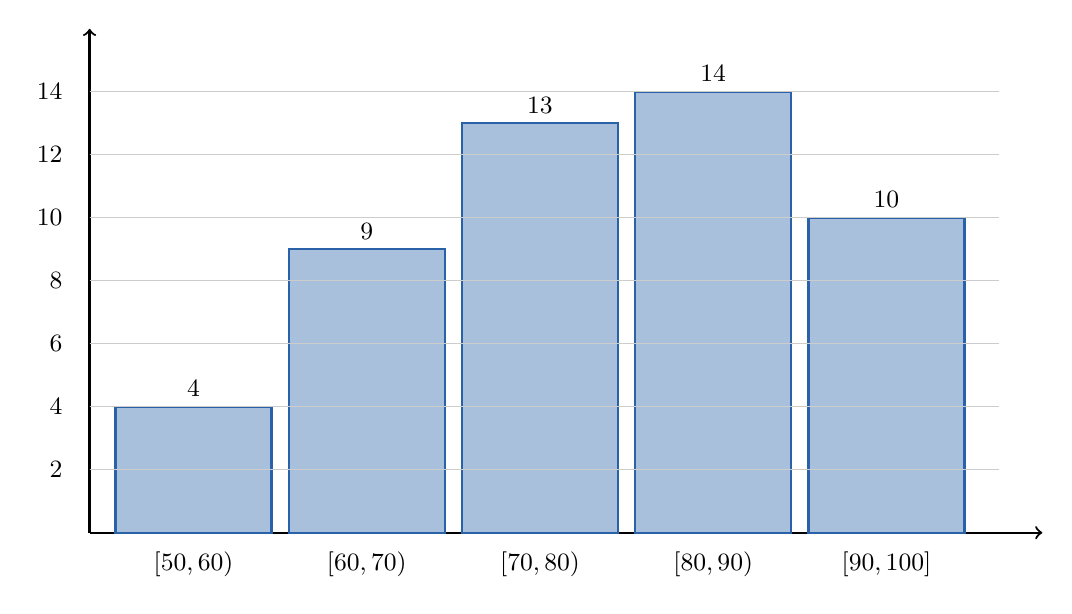
\begin{tikzpicture}[xscale=1.1, yscale=0.4]
  % 坐标轴
  \draw[->,thick] (0,0) -- (11,0);
  \draw[->,thick] (0,0) -- (0,16);
  % 柱状图（频数：4, 9, 13, 14, 10）
  \fill[mainblue!40,draw=mainblue, thick] (0.3,0) rectangle (2.1,4);
  \fill[mainblue!40,draw=mainblue, thick] (2.3,0) rectangle (4.1,9);
  \fill[mainblue!40,draw=mainblue, thick] (4.3,0) rectangle (6.1,13);
  \fill[mainblue!40,draw=mainblue, thick] (6.3,0) rectangle (8.1,14);
  \fill[mainblue!40,draw=mainblue, thick] (8.3,0) rectangle (10.1,10);
  % 频数标注
  \node[above,font=\small] at (1.2,4) {4};
  \node[above,font=\small] at (3.2,9) {9};
  \node[above,font=\small] at (5.2,13) {13};
  \node[above,font=\small] at (7.2,14) {14};
  \node[above,font=\small] at (9.2,10) {10};
  % x轴标签
  \node[below,font=\small] at (1.2,-0.3) {$[50,60)$};
  \node[below,font=\small] at (3.2,-0.3) {$[60,70)$};
  \node[below,font=\small] at (5.2,-0.3) {$[70,80)$};
  \node[below,font=\small] at (7.2,-0.3) {$[80,90)$};
  \node[below,font=\small] at (9.2,-0.3) {$[90,100]$};
  % y轴刻度
  \foreach \y in {2,4,6,8,10,12,14} {
    \draw[gray!40] (0,\y) -- (10.5,\y);
    \node[left,font=\small] at (-0.2,\y) {\y};
  }
\end{tikzpicture}
\end{center}

从直方图可以看出，成绩主要集中在 $70 \sim 90$ 分之间。
\end{examplebox}

\begin{examplebox}[【例题4】绘制扇形图]
根据例题3的频数分布表，画出各分组的扇形图（饼图）。

\textbf{解：}

各分组对应的扇形圆心角度数：
\begin{itemize}[leftmargin=2em]
  \item $[50, 60)$：$0.08 \times 360° = 28.8°$
  \item $[60, 70)$：$0.18 \times 360° = 64.8°$
  \item $[70, 80)$：$0.26 \times 360° = 93.6°$
  \item $[80, 90)$：$0.28 \times 360° = 100.8°$
  \item $[90, 100]$：$0.20 \times 360° = 72°$
\end{itemize}

\begin{center}
\begin{tikzpicture}
\pie[
  radius=3,
  color={blue!30, green!40, orange!50, red!40, purple!40},
  text=legend,
  sum=auto,
  before number=\phantom{0},
  after number={人}
]{8/50--60分: 4人, 18/60--70分: 9人, 26/70--80分: 13人, 28/80--90分: 14人, 20/90--100分: 10人}
\end{tikzpicture}
\end{center}

（注：上图中百分比 = 频率 $\times 100\%$）
\end{examplebox}

\begin{examplebox}[【例题5】用样本估计总体]
某市有12000名初中毕业生参加中考。为了解数学成绩情况，随机抽取了200名考生的数学成绩，统计结果如下：

\begin{center}
\begin{tabular}{|c|c|}
\hline
成绩范围 & 频数 \\
\hline
90分以上 & 40 \\
\hline
$75 \sim 90$分 & 80 \\
\hline
$60 \sim 75$分 & 50 \\
\hline
60分以下 & 30 \\
\hline
\end{tabular}
\end{center}

（1）估计该市成绩在90分以上的考生约有多少人？

（2）估计该市及格（60分及以上）的考生约有多少人？

\textbf{解：}

（1）样本中90分以上的频率为 $\dfrac{40}{200} = 0.20$

估计全市90分以上的考生约有 $12000 \times 0.20 = 2400$ 人。

（2）样本中及格（60分及以上）的频数为 $40 + 80 + 50 = 170$

频率为 $\dfrac{170}{200} = 0.85$

估计全市及格的考生约有 $12000 \times 0.85 = 10200$ 人。
\end{examplebox}

\begin{examplebox}[【例题6】统计图的综合分析]
下图是某班50名学生每天课外阅读时间的条形图和扇形图。请根据图形信息回答问题。

\textbf{条形图：}

\begin{center}
\begin{tikzpicture}
\begin{axis}[
  ybar,
  width=10cm, height=6cm,
  xlabel={每天阅读时间},
  ylabel={人数},
  ymin=0, ymax=25,
  xtick={1,2,3,4},
  xticklabels={不足30分钟,30--60分钟,60--90分钟,90分钟以上},
  x tick label style={rotate=15, font=\small},
  ytick={0,5,10,15,20,25},
  bar width=1.2cm,
  fill=mainblue!50,
  draw=mainblue,
  nodes near coords,
  nodes near coords style={font=\small},
]
\addplot coordinates {(1,8) (2,20) (3,15) (4,7)};
\end{axis}
\end{tikzpicture}
\end{center}

（1）阅读时间在"30--60分钟"的人数是多少？占全班的百分比是多少？

（2）阅读时间在60分钟以上（含60分钟）的学生有多少人？占全班的百分之几？

\textbf{解：}

（1）阅读时间在"30--60分钟"的人数为 \textbf{20人}，占全班的百分比为 $\dfrac{20}{50} \times 100\% = 40\%$。

（2）阅读时间在60分钟以上的人数为 $15 + 7 = 22$ 人。

占全班的百分比为 $\dfrac{22}{50} \times 100\% = 44\%$。
\end{examplebox}

\begin{examplebox}[【例题7】折线图的分析与趋势判断]
下图是某城市2020--2025年月平均气温的变化折线图（某月数据）。

\begin{center}
\begin{tikzpicture}
\begin{axis}[
  width=11cm, height=6cm,
  xlabel={年份},
  ylabel={月平均气温（$°C$）},
  ymin=15, ymax=28,
  xtick={2020,2021,2022,2023,2024,2025},
  ytick={16,18,20,22,24,26,28},
  grid=major,
  grid style={dashed, gray!30},
]
\addplot[thick, mainblue, mark=*, mark size=2.5pt] coordinates {
  (2020, 20) (2021, 21) (2022, 19) (2023, 23) (2024, 25) (2025, 24)
};
\end{axis}
\end{tikzpicture}
\end{center}

（1）哪一年的月平均气温最高？是多少？

（2）从2020年到2025年，气温总体呈什么趋势？

\textbf{解：}

（1）2024年的月平均气温最高，为 $25°C$。

（2）从2020年到2025年，气温总体呈\textbf{上升趋势}（2022年略有回落，2025年略有下降，但总体上升）。
\end{examplebox}

% ============ 第三部分：应用题 ============
\section*{\textcolor{apppurple}{三、应用题}}

\begin{appbox}[【应用1】学校食堂调查]
某校为了解学生对食堂饭菜的满意度，准备进行调查。全校共有2000名学生。

（1）你认为应该采用全面调查还是抽样调查？为什么？

（2）如果采用抽样调查，从每个年级随机抽取50名学生，共抽取150名学生进行问卷调查。结果如下：

\begin{center}
\begin{tabular}{|c|c|}
\hline
评价 & 人数 \\
\hline
非常满意 & 30 \\
\hline
满意 & 54 \\
\hline
一般 & 42 \\
\hline
不满意 & 18 \\
\hline
非常不满意 & 6 \\
\hline
\end{tabular}
\end{center}

请计算各评价的频率，并估计全校对食堂"满意"和"非常满意"的学生约有多少人。

\textbf{解：}

（1）应采用\textbf{抽样调查}。因为全校有2000名学生，人数较多，全面调查耗时耗力，且不必要对每人进行调查。抽样调查省时省力，且样本具有代表性。

（2）各评价的频率：

\begin{center}
\begin{tabular}{|c|c|c|}
\hline
评价 & 人数 & 频率 \\
\hline
非常满意 & 30 & $30 \div 150 = 0.20$ \\
\hline
满意 & 54 & $54 \div 150 = 0.36$ \\
\hline
一般 & 42 & $42 \div 150 = 0.28$ \\
\hline
不满意 & 18 & $18 \div 150 = 0.12$ \\
\hline
非常不满意 & 6 & $6 \div 150 = 0.04$ \\
\hline
\end{tabular}
\end{center}

"满意"和"非常满意"的频率之和为 $0.20 + 0.36 = 0.56$

估计全校满意和非常满意的学生约有 $2000 \times 0.56 = 1120$ 人。
\end{appbox}

\begin{appbox}[【应用2】产品质量检测]
某工厂生产一批灯泡，共10000个。质检部门随机抽取了200个灯泡进行寿命测试，结果如下：

\begin{center}
\begin{tabular}{|c|c|}
\hline
寿命范围 & 频数 \\
\hline
不足500小时 & 6 \\
\hline
$500 \sim 800$小时 & 30 \\
\hline
$800 \sim 1000$小时 & 80 \\
\hline
$1000 \sim 1200$小时 & 54 \\
\hline
1200小时以上 & 30 \\
\hline
\end{tabular}
\end{center}

（1）估计这批灯泡中寿命不低于800小时的灯泡约有多少个？

（2）如果工厂承诺"寿命不足500小时的灯泡可免费更换"，估计需要更换多少个灯泡？

\textbf{解：}

（1）样本中寿命不低于800小时的频数为 $80 + 54 + 30 = 164$

频率为 $\dfrac{164}{200} = 0.82$

估计这批灯泡中寿命不低于800小时的约有 $10000 \times 0.82 = 8200$ 个。

（2）样本中寿命不足500小时的频率为 $\dfrac{6}{200} = 0.03$

估计需要更换的灯泡约有 $10000 \times 0.03 = 300$ 个。
\end{appbox}

\begin{appbox}[【应用3】健康数据分析]
某校为了解学生的视力情况，随机抽取了80名学生检测视力，结果如下：

\begin{center}
\begin{tabular}{|c|c|}
\hline
视力 & 人数 \\
\hline
5.0及以上（正常） & 32 \\
\hline
$4.8 \sim 4.9$（轻度近视） & 24 \\
\hline
$4.5 \sim 4.7$（中度近视） & 16 \\
\hline
4.5以下（重度近视） & 8 \\
\hline
\end{tabular}
\end{center}

（1）计算各视力等级的频率。

（2）若全校有1200名学生，估计视力正常的学生约有多少人？

（3）估计全校近视（视力低于5.0）的学生约有多少人？

（4）请根据以上数据画出扇形图。

\textbf{解：}

（1）各视力等级的频率：

\begin{center}
\begin{tabular}{|c|c|c|}
\hline
视力 & 人数 & 频率 \\
\hline
5.0及以上 & 32 & $32 \div 80 = 0.40$ \\
\hline
$4.8 \sim 4.9$ & 24 & $24 \div 80 = 0.30$ \\
\hline
$4.5 \sim 4.7$ & 16 & $16 \div 80 = 0.20$ \\
\hline
4.5以下 & 8 & $8 \div 80 = 0.10$ \\
\hline
\end{tabular}
\end{center}

（2）估计视力正常的学生约有 $1200 \times 0.40 = 480$ 人。

（3）近视学生的频率为 $0.30 + 0.20 + 0.10 = 0.60$

估计全校近视学生约有 $1200 \times 0.60 = 720$ 人。

（4）扇形图圆心角：

\begin{itemize}[leftmargin=2em]
  \item 5.0及以上：$0.40 \times 360° = 144°$
  \item $4.8 \sim 4.9$：$0.30 \times 360° = 108°$
  \item $4.5 \sim 4.7$：$0.20 \times 360° = 72°$
  \item 4.5以下：$0.10 \times 360° = 36°$
\end{itemize}

\begin{center}
\begin{tikzpicture}
\pie[
  radius=3,
  color={green!50, yellow!50, orange!50, red!50},
  text=legend,
  sum=auto,
  before number=\phantom{0},
  after number={人}
]{40/5.0及以上: 32人, 30/4.8--4.9: 24人, 20/4.5--4.7: 16人, 10/4.5以下: 8人}
\end{tikzpicture}
\end{center}
\end{appbox}

% ============ 第四部分：课堂练习 ============
\section*{\textcolor{tipgreen}{四、课堂练习}}

\begin{enumerate}[leftmargin=2em]
  \item 为了解一批电视机的使用寿命，从中抽取了50台进行测试。请指出总体、个体、样本和样本容量。

  \item 下表是某班40名学生最喜欢的体育运动的调查结果。请补全表格并画出条形图。

\begin{center}
\begin{tabular}{|c|c|c|}
\hline
运动项目 & 频数 & 频率 \\
\hline
篮球 & 12 & \\
\hline
足球 & & 0.25 \\
\hline
乒乓球 & 8 & \\
\hline
其他 & & \\
\hline
\textbf{合计} & & \\
\hline
\end{tabular}
\end{center}

  \item 某校有800名学生，随机抽查了100名学生的课外阅读量（本/学期），得到频数分布表如下：

\begin{center}
\begin{tabular}{|c|c|}
\hline
阅读量（本） & 频数 \\
\hline
$[0, 5)$ & 10 \\
\hline
$[5, 10)$ & 30 \\
\hline
$[10, 15)$ & 35 \\
\hline
$[15, 20)$ & 20 \\
\hline
$[20, 25]$ & 5 \\
\hline
\end{tabular}
\end{center}

（1）计算各组的频率。

（2）估计全校课外阅读量在10本以上（含10本）的学生约有多少人？

  \item 判断下列调查分别适合用全面调查还是抽样调查：
\begin{enumerate}[label=(\arabic*)]
  \item 了解全国七年级学生的视力状况
  \item 检查一批导弹的杀伤半径
  \item 了解某班同学的身高
  \item 调查某电视节目的收视率
\end{enumerate}

  \item 某市环保局对该市5000辆汽车的尾气排放进行检测，随机抽取了250辆，其中不合格的有25辆。估计该市尾气不合格的汽车约有多少辆？
\end{enumerate}

\vspace{20pt}

\begin{knowledgebox}[参考答案]
\textbf{第1题：}
\begin{itemize}[leftmargin=2em]
  \item 总体：这批电视机的使用寿命
  \item 个体：每台电视机的使用寿命
  \item 样本：被抽取的50台电视机的使用寿命
  \item 样本容量：50
\end{itemize}

\textbf{第2题：}

足球频数 $= 40 \times 0.25 = 10$；其他频数 $= 40 - 12 - 10 - 8 = 10$

\begin{center}
\begin{tabular}{|c|c|c|}
\hline
运动项目 & 频数 & 频率 \\
\hline
篮球 & 12 & 0.30 \\
\hline
足球 & 10 & 0.25 \\
\hline
乒乓球 & 8 & 0.20 \\
\hline
其他 & 10 & 0.25 \\
\hline
\textbf{合计} & \textbf{40} & \textbf{1.00} \\
\hline
\end{tabular}
\end{center}

\begin{center}
\begin{tikzpicture}
\begin{axis}[
  ybar,
  width=9cm, height=5cm,
  xlabel={运动项目},
  ylabel={人数},
  ymin=0, ymax=16,
  xtick={1,2,3,4},
  xticklabels={篮球,足球,乒乓球,其他},
  bar width=1.5cm,
  fill=mainblue!50,
  draw=mainblue,
  nodes near coords,
]
\addplot coordinates {(1,12) (2,10) (3,8) (4,10)};
\end{axis}
\end{tikzpicture}
\end{center}

\textbf{第3题：}

（1）各组频率：$0.10$，$0.30$，$0.35$，$0.20$，$0.05$

（2）10本以上的频率为 $0.35 + 0.20 + 0.05 = 0.60$

估计全校约有 $800 \times 0.60 = 480$ 人。

\textbf{第4题：}
\begin{enumerate}[label=(\arabic*)]
  \item 抽样调查（范围太大）
  \item 抽样调查（具有破坏性）
  \item 全面调查（范围小，无破坏性）
  \item 抽样调查（范围太大）
\end{enumerate}

\textbf{第5题：}样本中不合格率为 $\dfrac{25}{250} = 0.10$

估计该市尾气不合格的汽车约有 $5000 \times 0.10 = 500$ 辆。
\end{knowledgebox}

\vfill
\begin{center}
\small\textcolor{gray}{本讲义仅供教学参考，例题可根据学生水平调整难度。}
\end{center}

\end{document}
